\documentclass{article}

\usepackage[utf8]{inputenc}
\usepackage{graphicx} 
\usepackage{booktabs} 
\usepackage{hyperref} 
\usepackage{float}
\usepackage{caption}
\usepackage{amsmath}

\title{the Impact of News Information Acquisition and Cognition}
\author{Chuanyi You\\Chuyi Zheng\\Cunyu Zhang\\Zixuan Yang}
\date{\today}

\begin{document}

\maketitle
\tableofcontents
\newpage

\section{Background}

In contemporary society, the proliferation of news and information acquisition channels has had a profound impact on individual social attitudes and cognitive behaviors. The "2019 College Students' Social Mentality Survey," led by Dr. Ma Deyong, a professor of political science at Renmin University of China, is designed to explore how Chinese college students access news and information and the subsequent effect on their perception of societal, political, and economic issues.

This survey spans a comprehensive range of topics, from basic demographic information of respondents, such as age, gender, and educational background, to their satisfaction with the country's political and economic state, and their trust and preference towards various news media channels. It also delves into students' interest in political news, the amount of time they spend on such news, and their views on the challenges faced by media outlets in delivering truthful reporting.

The research based on the survey aims to explore the impact of consuming political news on college students' perceptions and sentiments about the current state of society.

\section{Data}
The data set from the "2019 College Student Information Perception Survey" contains 1,254 entries and 133 columns, indicating a comprehensive set of questions addressed in the survey. 

\subsection{Data Processing}
Within the data set, questions 2 to 9 solicit personal information from respondents, such as age, gender, political affiliation, highest educational qualification, academic institution tier, field of study, family annual income, and hometown location. These variables will serve as control variables in the research. Questions 10, 11, and 12 investigate the respondents' satisfaction levels regarding politics, the economy, and personal life, respectively. These will act as dependent variables to assess the students' cognition. Questions 13, 14, and 15 explore the independent variables of interest for our research question, specifically the college students' interest in political news, the time spent browsing news, and the channels used for news consumption. The news channels variable is further processed into a binary variable indicating whether respondents access foreign media and their websites. Responses with a completion time of less than ten minutes will be excluded from the analysis. Question 31 serves as a mechanism to identify and eliminate responses from participants who do not answer the survey earnestly. The study does not encompass the survey questions such as college students' personal sentiments and their opinions on the news. Age column is also  removed since the respondenta are all college students.
\subsection{Descriptive Data}
\begin{figure}[H]
\centering
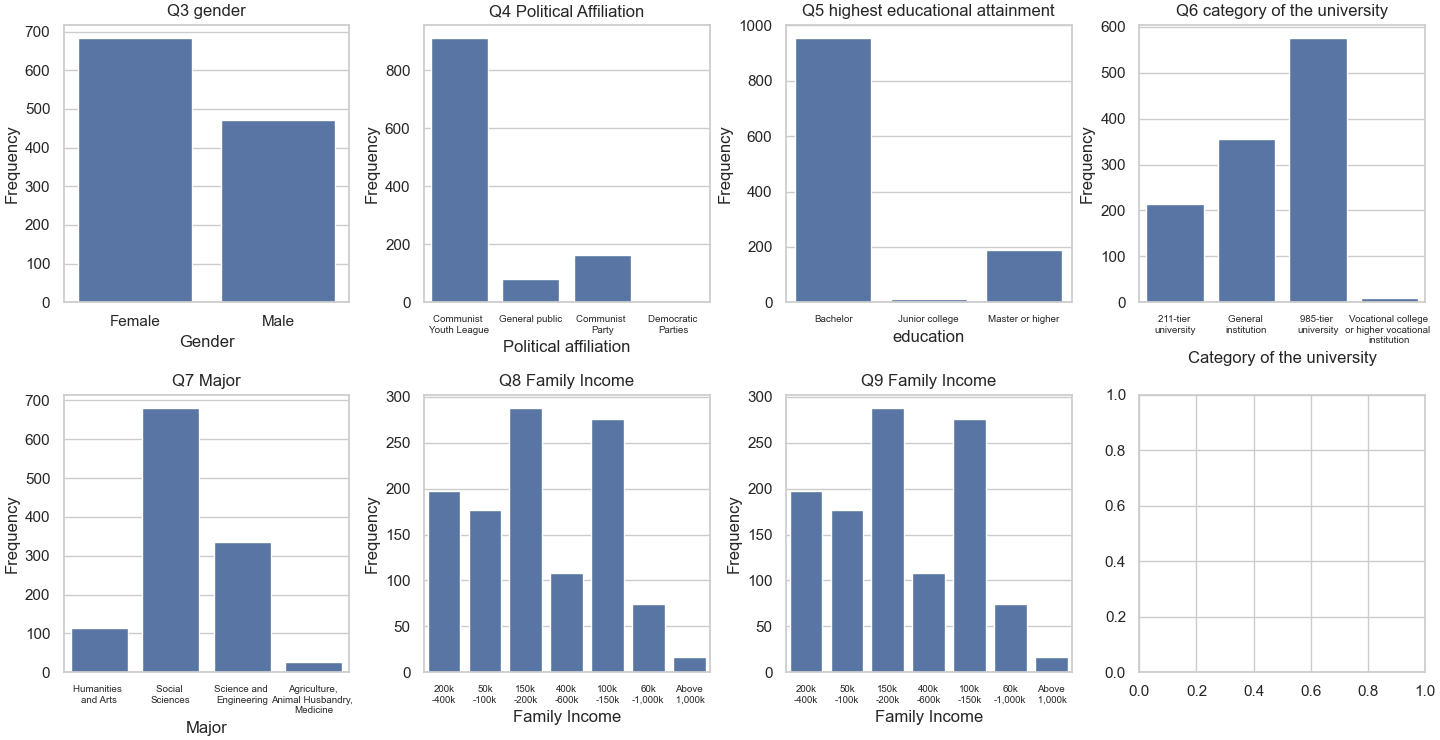
\includegraphics[width=\textwidth]{Figure_1.png}
\caption{Distribution regarding questions 2 to 9, information from respondents, such as age, gender, political affiliation, highest educational qualification, academic institution tier, field of study, family annual income, and hometown location. }
\label{fig:Control Variables}
\end{figure}
In the presented data, the gender distribution shows a slight majority of female respondents over males. Political affiliations lean significantly toward the Communist Youth League, with smaller representations from members of the Communist Party. Educational attainment is predominantly at the bachelor's level, with a smaller proportion holding a master's degree or higher. Considering university categories, the majority of respondents are from 985-tier universities, while vocational colleges account for fewer participants.

The major field of study is led by social sciences, followed by science and engineering. Agriculture, engineering, animal husbandry, and medicine have the smallest numbers of students.

The family income distribution reveals that most respondents come from families earning between 150k to 200k, with fewer in the 100k to 150k bracket. Most respondents are from small towns.


\begin{figure}[H]
\centering
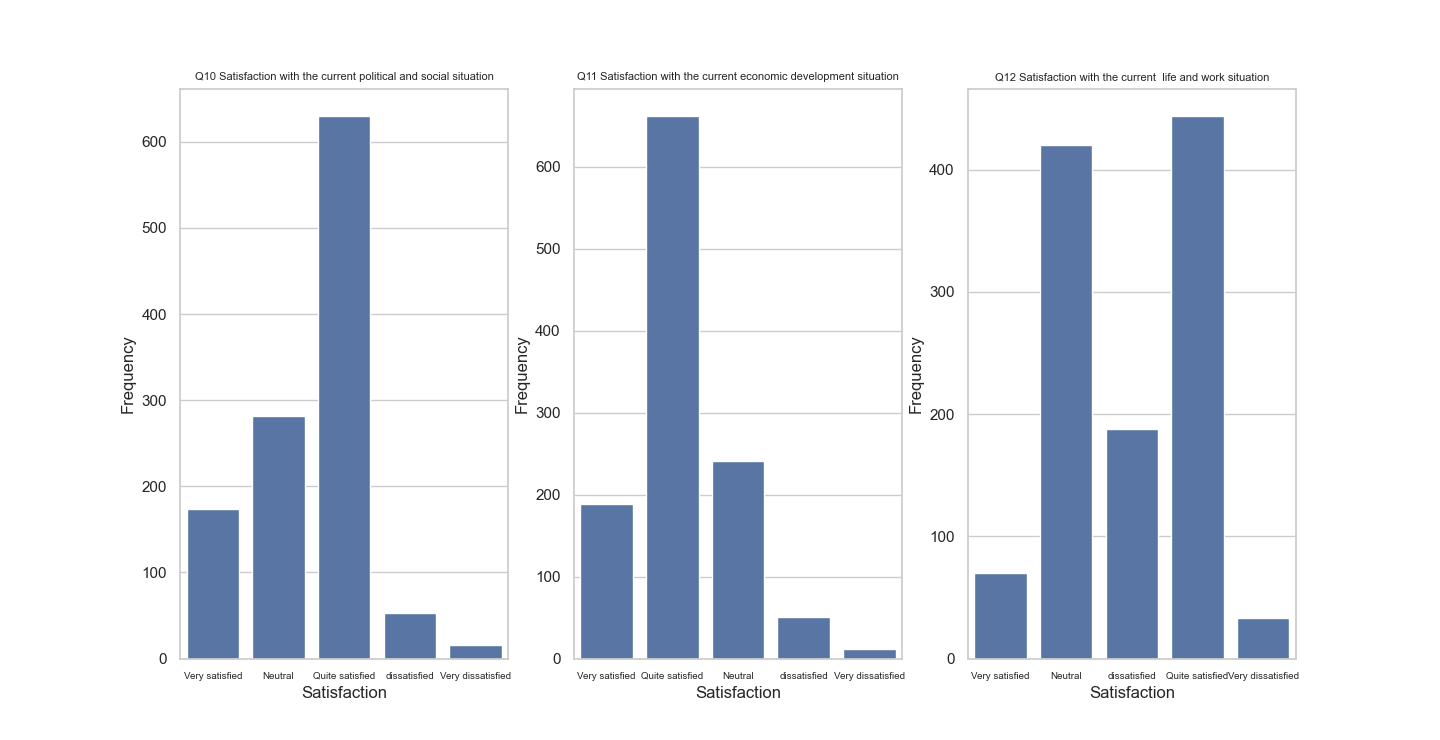
\includegraphics[width=\textwidth]{Figure_2.png}
\caption{Distribution regarding question 10, 11 and 12 investigate the respondents' satisfaction levels regarding politics, the economy, and personal life.}
\label{fig:Dependent variables}
\end{figure}
Satisfaction levels with the current political and social situation, economic development, situations show a trend towards quite satisfied, with a reasonable distribution across the satisfaction spectrum. However, when it comes to personal situation, more people showed their dissatisfaction.
\begin{figure}[H]
\centering
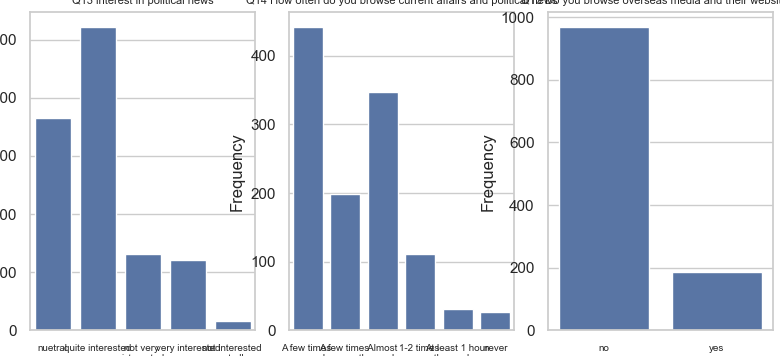
\includegraphics[width=\textwidth]{Figure_3.png}
\caption{Distribution regarding question 12, 13 and 14 investigate the respondents' interest in political news, the time spent browsing news, and the channels used for news consumption}
\label{fig:independent variables}
\end{figure}
Interest in political news is predominantly quite interested to neutral, with very few indicating extreme disinterest. The frequency of browsing current affairs and political news is highest for a few times per week, followed by almost everyday. Finally, the majority of respondents do not browse overseas media and their websites.
\section{Hypothesis}



\subsection{Regression}
\begin{equation}
\begin{aligned}
\text{pol\_sat} &= \beta_0 + \beta_1 \cdot \text{interest} + \beta_2 \cdot \text{time} + \beta_3 \cdot \text{overseas} + \gamma \cdot \text{controls} + \epsilon_1 \nonumber \\
\text{eco\_sati} &= \beta_0 + \beta_1 \cdot \text{interest} + \beta_2 \cdot \text{time} + \beta_3 \cdot \text{overseas} + \gamma \cdot \text{controls} + \epsilon_2 \nonumber \\
\text{lif\_work\_sati} &= \beta_0 + \beta_1 \cdot \text{interest} + \beta_2 \cdot \text{time} + \beta_3 \cdot \text{overseas} + \gamma \cdot \text{controls} + \epsilon_3 \nonumber
\end{aligned}
\end{equation}

\vspace{\baselineskip}
Where,
\begin{align*}
\text{pol\_sat} & : \text{Political satisfaction} \\
\text{eco\_sati} & : \text{Economic satisfaction} \\
\text{lif\_work\_sati} & : \text{Life and work satisfaction} \\
\beta_0 & :\text{intercept} \\
\beta_1, \beta_2, \beta_3 & : \text{Regression coefficients} \\
\gamma & : \text{Coefficient for the control variables} \\
\text{controls} & : \text{Vector of control variables} \\
\epsilon_1, \epsilon_2, \epsilon_3 & : \text{Error terms, unexplained factors in the model}
\end{align*}

We constructed three regression models to explore the determinants of political satisfaction (pol\_sat), economic satisfaction (eco\_sati), and life work satisfaction (lif\_work\_sati). These models integrate respondents' demographic details, including age, gender, political affiliation, highest level of education, institution level, field of study, annual household income, and hometown, as control variables.

Moreover, the models incorporate individual factors such as interest in political news, time allocation, and exposure to overseas information as explanatory variables. The aim is to comprehensively investigate satisfaction levels in the domains of politics, economics, and life\&work, considering a spectrum of personal and behavioral aspects. This modeling approach establishes a robust framework for a nuanced understanding of the factors influencing individuals' satisfaction levels.
\vspace{\baselineskip}
\vspace{\baselineskip}
\vspace{\baselineskip}
\subsection{Robustness}
For the robustness check, an ordered logistic regression model is employed.

\begin{align}
\text{Logit}(P(\text{pol\_sati} \leq j)) &= \alpha_j + \beta_1 \cdot \text{interest} + \beta_2 \cdot \text{time} + \beta_3 \cdot \text{overseas} + \gamma \cdot \text{controls} \nonumber \\
\text{Logit}(P(\text{eco\_sati} \leq j)) &= \alpha_j + \beta_1 \cdot \text{interest} + \beta_2 \cdot \text{time} + \beta_3 \cdot \text{overseas} + \gamma \cdot \text{controls} \nonumber \\
\text{Logit}(P(\text{lif\_work\_sati} \leq j)) &= \alpha_j + \beta_1 \cdot \text{interest} + \beta_2 \cdot \text{time} + \beta_3 \cdot \text{overseas} + \gamma \cdot \text{controls} \nonumber
\end{align}

\vspace{\baselineskip}
Where,
\begin{align*}
\text{Logit}(P(\text{pol\_sati} \leq j)) & : \text{Ordered log-odds for political satisfaction} \\
\text{Logit}(P(\text{eco\_sati} \leq j)) & : \text{Ordered log-odds for economic satisfaction} \\
\text{Logit}(P(\text{lif\_work\_sati} \leq j)) & : \text{Ordered log-odds for life and work satisfaction} \\
\alpha_j & : \text{Threshold parameters for different levels of satisfaction} \\
\beta_1, \beta_2, \beta_3 & : \text{Regression coefficients} \\
\gamma & : \text{Coefficient for the control variables} \\
\text{controls} & : \text{Vector of control variables}
\end{align*}

Here, each equation represents an ordered logit model of political satisfaction, economic satisfaction, and life\&work satisfaction at different satisfaction levels. The model covers threshold parameters ($\alpha_j$), regression coefficients ($\beta_1, \beta_2, \beta_3$) reflecting the effects of explanatory variables, and coefficients of control variables ($\gamma$) for each satisfaction level.

In this way, we are able to check the consistency of the estimated coefficients under different specifications and thus assess the robustness of the results. The inclusion of control variables ensures that any observed effects are robust to bias due to omitted variables
\section{Results}
\subsection{OLS Regression}
\begin{table}[H]
  \centering
  \caption{Regression Results for Dependent Variable Q10}\label{tab:regression_q10}
  \begin{tabular}{lcccccc}
    \toprule
    \textbf{Variable} & \textbf{Coefficient} & \textbf{Std. Error} & \textbf{t-value} & \textbf{P-value} & \textbf{[0.025} & \textbf{0.975]} \\
    \midrule
    const   & 4.7176 & 0.296 & 15.914 & 0.000 & 4.136 & 5.299 \\
    Q3      & -0.0273 & 0.051 & -0.537 & 0.592 & -0.127 & 0.072 \\
    Q4      & 0.0696 & 0.024 & 2.889 & 0.004 & 0.022 & 0.117 \\
    Q6      & 0.0122 & 0.027 & 0.448 & 0.654 & -0.041 & 0.066 \\
    Q7      & 0.1430 & 0.038 & 3.748 & 0.000 & 0.068 & 0.218 \\
    Q8      & -0.0140 & 0.016 & -0.869 & 0.385 & -0.046 & 0.018 \\
    Q9      & -0.0273 & 0.019 & -1.410 & 0.159 & -0.065 & 0.011 \\
    Q13     & 0.1652 & 0.034 & 4.883 & 0.000 & 0.099 & 0.232 \\
    Q14     & -0.0216 & 0.028 & -0.785 & 0.432 & -0.076 & 0.032 \\
    Q15\_A8 & -0.3604 & 0.065 & -5.555 & 0.000 & -0.488 & -0.233 \\
    \bottomrule
  \end{tabular}
\end{table}

The findings in Table 1 reveal that the p-values associated with all three explanatory variables are below the conventional significance threshold of 0.05. This suggests that each of these variables is statistically significant. Specifically, the coefficient for Q13 (interest in political news) is estimated at 0.1652. This implies that, while keeping all other variables constant, a one-unit increase in students' interest in political news corresponds to a 0.1652 unit rise in their satisfaction with politics (pol\_sati). Q14 has a coefficient of indicates that the more frequently political news is read, political satisfaction decreases by 0.0237 units. Similarly, the more exposure to overseas news, the less satisfied they are with politics, decreasing by 0.1993 units.
\vspace{\baselineskip}
\begin{table}[H]
  \centering
  \caption{Regression Results for Dependent Variable Q11}\label{tab:regression_q11}
  \begin{tabular}{lcccccc}
    \toprule
    \textbf{Variable} & \textbf{Coefficient} & \textbf{Std. Error} & \textbf{t-value} & \textbf{P-value} & \textbf{[0.025} & \textbf{0.975]} \\
    \midrule
    const   & 5.2327 & 0.292 & 17.939 & 0.000 & 4.660 & 5.805 \\
    Q3      & -0.0072 & 0.050 & -0.145 & 0.885 & -0.105 & 0.091 \\
    Q4      & 0.0486 & 0.024 & 2.051 & 0.041 & 0.002 & 0.095 \\
    Q6      & -0.0161 & 0.027 & -0.601 & 0.548 & -0.069 & 0.036 \\
    Q7      & 0.1046 & 0.038 & 2.785 & 0.005 & 0.031 & 0.178 \\
    Q8      & -0.0250 & 0.016 & -1.574 & 0.116 & -0.056 & 0.006 \\
    Q9      & -0.0507 & 0.019 & -2.658 & 0.008 & -0.088 & -0.013 \\
    Q13     & 0.1451 & 0.033 & 4.360 & 0.000 & 0.080 & 0.210 \\
    Q14     & -0.0237 & 0.027 & -0.877 & 0.381 & -0.077 & 0.029 \\
    Q15\_A8 & -0.1993 & 0.064 & -3.122 & 0.002 & -0.325 & -0.074 \\
    \bottomrule
  \end{tabular}
\end{table}
According to results in Table 2, the positive coefficient of 0.1451 for Q13(interest in political news) suggests that, holding other variables constant, a one-unit increase in students' interest in political news is associated with a 0.1451 unit increase in satisfaction with economy. The coefficient for Q14 is -0.0237, indicating that there is no statistically significant relationship between time allocation (Q14) and satisfaction with economy, as the P-value is 0.381.The negative coefficient of -0.1993 for Q15\_A8 suggests that, holding other variables constant, a one-unit increase in exposure to overseas information is associated with a 0.1993 unit decrease in satisfaction with economy. The P-value of 0.002 indicates that this relationship is statistically significant.
\vspace{\baselineskip}
\begin{table}[H]
  \centering
  \caption{Regression Results for Dependent Variable Q12}\label{tab:regression_q12}
  \begin{tabular}{lcccccc}
    \toprule
    \textbf{Variable} & \textbf{Coefficient} & \textbf{Std. Error} & \textbf{t-value} & \textbf{P-value} & \textbf{[0.025} & \textbf{0.975]} \\
    \midrule
    const   & 4.5699 & 0.335 & 13.644 & 0.000 & 3.913 & 5.227 \\
    Q3      & -0.0330 & 0.057 & -0.575 & 0.566 & -0.146 & 0.080 \\
    Q4      & -0.0325 & 0.027 & -1.194 & 0.233 & -0.086 & 0.021 \\
    Q6      & -0.0150 & 0.031 & -0.488 & 0.625 & -0.075 & 0.045 \\
    Q7      & 0.0773 & 0.043 & 1.793 & 0.073 & -0.007 & 0.162 \\
    Q8      & 0.0450 & 0.018 & 2.468 & 0.014 & 0.009 & 0.081 \\
    Q9      & -0.0670 & 0.022 & -3.061 & 0.002 & -0.110 & -0.024 \\
    Q13     & 0.1974 & 0.038 & 5.164 & 0.000 & 0.122 & 0.272 \\
    Q14     & -0.0371 & 0.031 & -1.194 & 0.233 & -0.098 & 0.024 \\
    Q15\_A8 & -0.1233 & 0.073 & -1.682 & 0.093 & -0.267 & 0.020 \\
    \bottomrule
  \end{tabular}
\end{table}
The results in Table 3 provide insights into the coefficients of the explanatory variables Q13, Q14, and Q15\_A8 for the dependent variable Q12(life\&work satisfaction).The positive coefficient of 0.1974 for Q13 suggests that, holding other variables constant, a one-unit increase in students' interest in political news is associated with a 0.1974 unit increase in satisfaction with life\&work.The coefficient for Q14 is -0.0371, indicating that there is no statistically significant relationship between time allocation (Q14) and satisfaction with life\&work, as the P-value is 0.233.The negative coefficient of -0.1233 for Q15\_A8 suggests that, holding other variables constant, a one-unit increase in exposure to overseas information is associated with a 0.1233 unit decrease in satisfaction with life\&work. The P-value of 0.093 indicates a marginal level of significance.
\newpage
\section{Conclusion}
\subsection{Political Satisfaction}
Interest in political news (Q13) has a positive effect on political satisfaction, with a coefficient of 0.1652. This means for every unit increase in interest in political news, political satisfaction increases by 0.1652 units, holding other variables constant.
Frequency of reading political news (Q14) has a slightly negative impact, decreasing political satisfaction by 0.0237 units for each unit increase in frequency.
Exposure to overseas news (Q15 A8) negatively impacts political satisfaction, with a coefficient of -0.1993. This suggests that more exposure to overseas news leads to a decrease in political satisfaction by 0.1993 units.
\subsection{Economic Satisfaction}
Interest in political news (Q13) positively correlates with economic satisfaction, with a coefficient of 0.1451. An increase in interest in political news leads to a 0.1451 unit increase in economic satisfaction.
The time spent on news (Q14) does not have a statistically significant relationship with economic satisfaction, as indicated by the non-significant P-value.
Exposure to overseas news (Q15 A8) has a significant negative effect, with a coefficient of -0.1993. More exposure to overseas news decreases satisfaction with the economy by 0.1993 units.
\subsection{Life and Work Satisfaction}
Interest in political news (Q13) shows a positive correlation, with a coefficient of 0.1974. This implies that an increase in interest in political news is associated with a 0.1974 unit increase in satisfaction with life and work.
The time allocated to news (Q14) does not show a significant relationship with life and work satisfaction.
Exposure to overseas news (Q15 A8) has a negative impact, with a coefficient of -0.1233. Increasing exposure to overseas news is associated with a decrease in life and work satisfaction by 0.1233 units, although this relationship has a marginal level of significance

\newpage
\section{Appendix}
\subsection{Odered Logistics Regression}
\begin{center}
\begin{tabular}{lclc}
\toprule
\textbf{Dep. Variable:}   &       Q10        & \textbf{  No. Observations:  } &     1155    \\
\textbf{Model:}           &     MNLogit      & \textbf{  Df Residuals:      } &     1111    \\
\textbf{Method:}          &       MLE        & \textbf{  Df Model:          } &       40    \\
\textbf{Date:}            & Mon, 04 Dec 2023 & \textbf{  Pseudo R-squ.:     } &  0.06228    \\
\textbf{Time:}            &     17:18:05     & \textbf{  Log-Likelihood:    } &   -1257.1   \\
\textbf{converged:}       &       True       & \textbf{  LL-Null:           } &   -1340.6   \\
\textbf{Covariance Type:} &    nonrobust     & \textbf{  LLR p-value:       } & 1.894e-17   \\
\bottomrule
\end{tabular}
\begin{tabular}{ccccccc}
 \textbf{Q10=4}  & \textbf{coef} & \textbf{std err} & \textbf{z} & \textbf{P$> |$z$|$} & \textbf{[0.025} & \textbf{0.975]}  \\
\midrule
\bottomrule
\end{tabular}
\begin{tabular}{lcccccc}
\textbf{const}   &      -5.6108  &        4.275     &    -1.312  &         0.189        &      -13.990    &        2.768     \\
\textbf{Q3}      &       0.0346  &        0.624     &     0.055  &         0.956        &       -1.189    &        1.258     \\
\textbf{Q4}      &      -0.2304  &        0.304     &    -0.758  &         0.449        &       -0.826    &        0.366     \\
\textbf{Q5}      &       1.4939  &        0.973     &     1.535  &         0.125        &       -0.414    &        3.402     \\
\textbf{Q6}      &       0.5038  &        0.382     &     1.317  &         0.188        &       -0.246    &        1.253     \\
\textbf{Q7}      &      -0.3887  &        0.507     &    -0.767  &         0.443        &       -1.382    &        0.605     \\
\textbf{Q8}      &       0.2255  &        0.188     &     1.199  &         0.231        &       -0.143    &        0.594     \\
\textbf{Q9}      &       0.5887  &        0.254     &     2.321  &         0.020        &        0.092    &        1.086     \\
\textbf{Q13}     &      -0.2408  &        0.438     &    -0.550  &         0.582        &       -1.099    &        0.617     \\
\textbf{Q14}     &       0.2473  &        0.364     &     0.680  &         0.497        &       -0.466    &        0.961     \\
\textbf{Q15\_A8} &       0.3588  &        0.669     &     0.536  &         0.592        &       -0.953    &        1.671     \\
\bottomrule
\end{tabular}
\begin{tabular}{ccccccc}
 \textbf{Q10=5}  & \textbf{coef} & \textbf{std err} & \textbf{z} & \textbf{P$> |$z$|$} & \textbf{[0.025} & \textbf{0.975]}  \\
\midrule
\bottomrule
\end{tabular}
\begin{tabular}{lcccccc}
\textbf{const}   &      -3.1491  &        3.870     &    -0.814  &         0.416        &      -10.734    &        4.436     \\
\textbf{Q3}      &       0.4110  &        0.565     &     0.727  &         0.467        &       -0.696    &        1.518     \\
\textbf{Q4}      &       0.0613  &        0.284     &     0.216  &         0.829        &       -0.495    &        0.618     \\
\textbf{Q5}      &       1.3222  &        0.925     &     1.429  &         0.153        &       -0.491    &        3.136     \\
\textbf{Q6}      &       0.4072  &        0.347     &     1.172  &         0.241        &       -0.274    &        1.088     \\
\textbf{Q7}      &      -0.2164  &        0.451     &    -0.480  &         0.631        &       -1.100    &        0.667     \\
\textbf{Q8}      &       0.0773  &        0.172     &     0.450  &         0.653        &       -0.259    &        0.414     \\
\textbf{Q9}      &       0.6099  &        0.229     &     2.661  &         0.008        &        0.161    &        1.059     \\
\textbf{Q13}     &      -0.3018  &        0.394     &    -0.767  &         0.443        &       -1.073    &        0.469     \\
\textbf{Q14}     &       0.0934  &        0.325     &     0.288  &         0.774        &       -0.544    &        0.730     \\
\textbf{Q15\_A8} &      -0.3195  &        0.612     &    -0.522  &         0.602        &       -1.520    &        0.881     \\
\bottomrule
\end{tabular}
\newpage
\begin{tabular}{ccccccc}
 \textbf{Q10=6}  & \textbf{coef} & \textbf{std err} & \textbf{z} & \textbf{P$> |$z$|$} & \textbf{[0.025} & \textbf{0.975]}  \\
\midrule
\bottomrule
\end{tabular}
\begin{tabular}{lcccccc}
\textbf{const}   &      -4.4936  &        3.825     &    -1.175  &         0.240        &      -11.990    &        3.002     \\
\textbf{Q3}      &       0.3822  &        0.556     &     0.688  &         0.492        &       -0.707    &        1.472     \\
\textbf{Q4}      &       0.1868  &        0.280     &     0.666  &         0.505        &       -0.363    &        0.737     \\
\textbf{Q5}      &       1.0665  &        0.918     &     1.161  &         0.245        &       -0.733    &        2.866     \\
\textbf{Q6}      &       0.3446  &        0.343     &     1.005  &         0.315        &       -0.328    &        1.017     \\
\textbf{Q7}      &      -0.0645  &        0.445     &    -0.145  &         0.885        &       -0.936    &        0.807     \\
\textbf{Q8}      &       0.1600  &        0.168     &     0.950  &         0.342        &       -0.170    &        0.490     \\
\textbf{Q9}      &       0.5620  &        0.226     &     2.490  &         0.013        &        0.120    &        1.004     \\
\textbf{Q13}     &       0.0530  &        0.388     &     0.137  &         0.891        &       -0.708    &        0.814     \\
\textbf{Q14}     &       0.1153  &        0.321     &     0.360  &         0.719        &       -0.513    &        0.744     \\
\textbf{Q15\_A8} &      -1.1108  &        0.603     &    -1.843  &         0.065        &       -2.292    &        0.070     \\
\bottomrule
\end{tabular}
\begin{tabular}{ccccccc}
 \textbf{Q10=7}  & \textbf{coef} & \textbf{std err} & \textbf{z} & \textbf{P$> |$z$|$} & \textbf{[0.025} & \textbf{0.975]}  \\
\midrule
\bottomrule
\end{tabular}
\begin{tabular}{lcccccc}
\textbf{const}   &      -4.6663  &        3.972     &    -1.175  &         0.240        &      -12.451    &        3.119     \\
\textbf{Q3}      &       0.0199  &        0.573     &     0.035  &         0.972        &       -1.104    &        1.144     \\
\textbf{Q4}      &       0.0615  &        0.289     &     0.213  &         0.831        &       -0.504    &        0.627     \\
\textbf{Q5}      &       0.3300  &        0.949     &     0.348  &         0.728        &       -1.529    &        2.189     \\
\textbf{Q6}      &       0.3426  &        0.353     &     0.972  &         0.331        &       -0.348    &        1.034     \\
\textbf{Q7}      &       0.3772  &        0.459     &     0.822  &         0.411        &       -0.522    &        1.277     \\
\textbf{Q8}      &      -0.0079  &        0.175     &    -0.045  &         0.964        &       -0.350    &        0.335     \\
\textbf{Q9}      &       0.3582  &        0.231     &     1.548  &         0.122        &       -0.095    &        0.812     \\
\textbf{Q13}     &       0.5401  &        0.402     &     1.343  &         0.179        &       -0.248    &        1.328     \\
\textbf{Q14}     &       0.0384  &        0.330     &     0.116  &         0.908        &       -0.609    &        0.686     \\
\textbf{Q15\_A8} &      -1.1602  &        0.632     &    -1.836  &         0.066        &       -2.398    &        0.078     \\
\bottomrule
\end{tabular}
%\caption{MNLogit Regression Results}
\end{center}
\newpage
\begin{center}
\begin{tabular}{lclc}
\toprule
\textbf{Dep. Variable:}   &       Q11        & \textbf{  No. Observations:  } &     1155    \\
\textbf{Model:}           &     MNLogit      & \textbf{  Df Residuals:      } &     1111    \\
\textbf{Method:}          &       MLE        & \textbf{  Df Model:          } &       40    \\
\textbf{Date:}            & Mon, 04 Dec 2023 & \textbf{  Pseudo R-squ.:     } &  0.04464    \\
\textbf{Time:}            &     17:18:05     & \textbf{  Log-Likelihood:    } &   -1244.0   \\
\textbf{converged:}       &       True       & \textbf{  LL-Null:           } &   -1302.2   \\
\textbf{Covariance Type:} &    nonrobust     & \textbf{  LLR p-value:       } & 2.300e-09   \\
\bottomrule
\end{tabular}
\begin{tabular}{ccccccc}
 \textbf{Q11=4}  & \textbf{coef} & \textbf{std err} & \textbf{z} & \textbf{P$> |$z$|$} & \textbf{[0.025} & \textbf{0.975]}  \\
\midrule
\bottomrule
\end{tabular}
\begin{tabular}{lcccccc}
\textbf{const}   &       3.1004  &        5.410     &     0.573  &         0.567        &       -7.504    &       13.705     \\
\textbf{Q3}      &       0.1224  &        0.697     &     0.176  &         0.861        &       -1.244    &        1.489     \\
\textbf{Q4}      &      -0.2866  &        0.377     &    -0.759  &         0.448        &       -1.026    &        0.453     \\
\textbf{Q5}      &       0.0862  &        0.899     &     0.096  &         0.924        &       -1.675    &        1.848     \\
\textbf{Q6}      &       0.2204  &        0.421     &     0.523  &         0.601        &       -0.605    &        1.046     \\
\textbf{Q7}      &      -0.0275  &        0.608     &    -0.045  &         0.964        &       -1.220    &        1.164     \\
\textbf{Q8}      &      -0.0576  &        0.202     &    -0.285  &         0.776        &       -0.454    &        0.339     \\
\textbf{Q9}      &       0.2819  &        0.280     &     1.007  &         0.314        &       -0.267    &        0.831     \\
\textbf{Q13}     &      -0.4740  &        0.521     &    -0.910  &         0.363        &       -1.495    &        0.547     \\
\textbf{Q14}     &       0.0166  &        0.431     &     0.038  &         0.969        &       -0.828    &        0.861     \\
\textbf{Q15\_A8} &       0.4532  &        0.741     &     0.611  &         0.541        &       -1.000    &        1.906     \\
\bottomrule
\end{tabular}
\begin{tabular}{ccccccc}
 \textbf{Q11=5}  & \textbf{coef} & \textbf{std err} & \textbf{z} & \textbf{P$> |$z$|$} & \textbf{[0.025} & \textbf{0.975]}  \\
\midrule
\bottomrule
\end{tabular}
\begin{tabular}{lcccccc}
\textbf{const}   &       9.1891  &        5.056     &     1.817  &         0.069        &       -0.721    &       19.099     \\
\textbf{Q3}      &       0.3322  &        0.646     &     0.514  &         0.607        &       -0.934    &        1.599     \\
\textbf{Q4}      &      -0.1719  &        0.359     &    -0.479  &         0.632        &       -0.876    &        0.532     \\
\textbf{Q5}      &      -0.5712  &        0.847     &    -0.674  &         0.500        &       -2.232    &        1.090     \\
\textbf{Q6}      &       0.0590  &        0.392     &     0.151  &         0.880        &       -0.709    &        0.828     \\
\textbf{Q7}      &      -0.0272  &        0.567     &    -0.048  &         0.962        &       -1.138    &        1.084     \\
\textbf{Q8}      &      -0.2380  &        0.187     &    -1.272  &         0.203        &       -0.605    &        0.129     \\
\textbf{Q9}      &       0.1370  &        0.258     &     0.531  &         0.596        &       -0.369    &        0.643     \\
\textbf{Q13}     &      -0.7502  &        0.487     &    -1.541  &         0.123        &       -1.704    &        0.204     \\
\textbf{Q14}     &      -0.0070  &        0.402     &    -0.017  &         0.986        &       -0.795    &        0.781     \\
\textbf{Q15\_A8} &      -0.1331  &        0.692     &    -0.192  &         0.848        &       -1.490    &        1.224     \\
\bottomrule
\end{tabular}
\newpage
\begin{tabular}{ccccccc}
 \textbf{Q11=6}  & \textbf{coef} & \textbf{std err} & \textbf{z} & \textbf{P$> |$z$|$} & \textbf{[0.025} & \textbf{0.975]}  \\
\midrule
\bottomrule
\end{tabular}
\begin{tabular}{lcccccc}
\textbf{const}   &       8.0718  &        4.996     &     1.616  &         0.106        &       -1.721    &       17.864     \\
\textbf{Q3}      &       0.2458  &        0.635     &     0.387  &         0.699        &       -0.999    &        1.490     \\
\textbf{Q4}      &      -0.1100  &        0.355     &    -0.310  &         0.757        &       -0.805    &        0.585     \\
\textbf{Q5}      &      -0.3556  &        0.832     &    -0.427  &         0.669        &       -1.987    &        1.275     \\
\textbf{Q6}      &      -0.0149  &        0.387     &    -0.039  &         0.969        &       -0.773    &        0.743     \\
\textbf{Q7}      &       0.0816  &        0.560     &     0.146  &         0.884        &       -1.016    &        1.179     \\
\textbf{Q8}      &      -0.2048  &        0.183     &    -1.118  &         0.263        &       -0.564    &        0.154     \\
\textbf{Q9}      &       0.1066  &        0.254     &     0.420  &         0.675        &       -0.391    &        0.604     \\
\textbf{Q13}     &      -0.3467  &        0.481     &    -0.721  &         0.471        &       -1.289    &        0.595     \\
\textbf{Q14}     &      -0.1133  &        0.397     &    -0.285  &         0.775        &       -0.891    &        0.665     \\
\textbf{Q15\_A8} &      -0.6449  &        0.677     &    -0.952  &         0.341        &       -1.973    &        0.683     \\
\bottomrule
\end{tabular}
\begin{tabular}{ccccccc}
 \textbf{Q11=7}  & \textbf{coef} & \textbf{std err} & \textbf{z} & \textbf{P$> |$z$|$} & \textbf{[0.025} & \textbf{0.975]}  \\
\midrule
\bottomrule
\end{tabular}
\begin{tabular}{lcccccc}
\textbf{const}   &       5.7370  &        5.108     &     1.123  &         0.261        &       -4.275    &       15.749     \\
\textbf{Q3}      &       0.1980  &        0.649     &     0.305  &         0.760        &       -1.074    &        1.470     \\
\textbf{Q4}      &      -0.0770  &        0.363     &    -0.212  &         0.832        &       -0.788    &        0.634     \\
\textbf{Q5}      &      -1.0804  &        0.864     &    -1.250  &         0.211        &       -2.774    &        0.613     \\
\textbf{Q6}      &      -0.0353  &        0.394     &    -0.090  &         0.929        &       -0.808    &        0.738     \\
\textbf{Q7}      &       0.4222  &        0.571     &     0.740  &         0.459        &       -0.696    &        1.541     \\
\textbf{Q8}      &      -0.2620  &        0.188     &    -1.394  &         0.163        &       -0.630    &        0.106     \\
\textbf{Q9}      &      -0.0707  &        0.259     &    -0.273  &         0.785        &       -0.578    &        0.437     \\
\textbf{Q13}     &       0.0957  &        0.491     &     0.195  &         0.845        &       -0.867    &        1.058     \\
\textbf{Q14}     &      -0.0351  &        0.405     &    -0.087  &         0.931        &       -0.829    &        0.759     \\
\textbf{Q15\_A8} &      -0.4741  &        0.696     &    -0.681  &         0.496        &       -1.838    &        0.890     \\
\bottomrule
\end{tabular}
%\caption{MNLogit Regression Results}
\end{center}
\newpage
\begin{center}
\begin{tabular}{lclc}
\toprule
\textbf{Dep. Variable:}   &       Q12        & \textbf{  No. Observations:  } &     1155    \\
\textbf{Model:}           &     MNLogit      & \textbf{  Df Residuals:      } &     1111    \\
\textbf{Method:}          &       MLE        & \textbf{  Df Model:          } &       40    \\
\textbf{Date:}            & Mon, 04 Dec 2023 & \textbf{  Pseudo R-squ.:     } &  0.03464    \\
\textbf{Time:}            &     17:18:05     & \textbf{  Log-Likelihood:    } &   -1452.1   \\
\textbf{converged:}       &       True       & \textbf{  LL-Null:           } &   -1504.2   \\
\textbf{Covariance Type:} &    nonrobust     & \textbf{  LLR p-value:       } & 1.255e-07   \\
\bottomrule
\end{tabular}
\begin{tabular}{ccccccc}
 \textbf{Q12=4}  & \textbf{coef} & \textbf{std err} & \textbf{z} & \textbf{P$> |$z$|$} & \textbf{[0.025} & \textbf{0.975]}  \\
\midrule
\bottomrule
\end{tabular}
\begin{tabular}{lcccccc}
\textbf{const}   &       7.6849  &        2.992     &     2.568  &         0.010        &        1.821    &       13.549     \\
\textbf{Q3}      &      -0.4900  &        0.436     &    -1.123  &         0.261        &       -1.345    &        0.365     \\
\textbf{Q4}      &      -0.1605  &        0.246     &    -0.652  &         0.514        &       -0.643    &        0.322     \\
\textbf{Q5}      &      -0.6997  &        0.550     &    -1.273  &         0.203        &       -1.777    &        0.377     \\
\textbf{Q6}      &      -0.0713  &        0.230     &    -0.310  &         0.757        &       -0.522    &        0.380     \\
\textbf{Q7}      &      -0.5006  &        0.304     &    -1.646  &         0.100        &       -1.097    &        0.096     \\
\textbf{Q8}      &      -0.2696  &        0.132     &    -2.043  &         0.041        &       -0.528    &       -0.011     \\
\textbf{Q9}      &      -0.0296  &        0.166     &    -0.178  &         0.859        &       -0.355    &        0.296     \\
\textbf{Q13}     &      -0.0362  &        0.272     &    -0.133  &         0.894        &       -0.570    &        0.497     \\
\textbf{Q14}     &      -0.0013  &        0.221     &    -0.006  &         0.995        &       -0.435    &        0.432     \\
\textbf{Q15\_A8} &      -0.4177  &        0.480     &    -0.871  &         0.384        &       -1.358    &        0.522     \\
\bottomrule
\end{tabular}
\begin{tabular}{ccccccc}
 \textbf{Q12=5}  & \textbf{coef} & \textbf{std err} & \textbf{z} & \textbf{P$> |$z$|$} & \textbf{[0.025} & \textbf{0.975]}  \\
\midrule
\bottomrule
\end{tabular}
\begin{tabular}{lcccccc}
\textbf{const}   &       7.0242  &        2.876     &     2.443  &         0.015        &        1.388    &       12.660     \\
\textbf{Q3}      &      -0.5194  &        0.418     &    -1.242  &         0.214        &       -1.339    &        0.300     \\
\textbf{Q4}      &      -0.2898  &        0.237     &    -1.225  &         0.221        &       -0.753    &        0.174     \\
\textbf{Q5}      &      -0.4363  &        0.519     &    -0.841  &         0.400        &       -1.453    &        0.581     \\
\textbf{Q6}      &      -0.0934  &        0.220     &    -0.425  &         0.671        &       -0.524    &        0.337     \\
\textbf{Q7}      &      -0.3963  &        0.291     &    -1.361  &         0.173        &       -0.967    &        0.174     \\
\textbf{Q8}      &      -0.1688  &        0.124     &    -1.358  &         0.175        &       -0.412    &        0.075     \\
\textbf{Q9}      &      -0.1233  &        0.159     &    -0.773  &         0.439        &       -0.436    &        0.189     \\
\textbf{Q13}     &       0.2459  &        0.261     &     0.940  &         0.347        &       -0.267    &        0.758     \\
\textbf{Q14}     &      -0.0435  &        0.212     &    -0.205  &         0.838        &       -0.460    &        0.373     \\
\textbf{Q15\_A8} &      -0.6690  &        0.454     &    -1.473  &         0.141        &       -1.559    &        0.221     \\
\bottomrule
\end{tabular}
\newpage
\begin{tabular}{ccccccc}
 \textbf{Q12=6}  & \textbf{coef} & \textbf{std err} & \textbf{z} & \textbf{P$> |$z$|$} & \textbf{[0.025} & \textbf{0.975]}  \\
\midrule
\bottomrule
\end{tabular}
\begin{tabular}{lcccccc}
\textbf{const}   &       4.3408  &        2.877     &     1.509  &         0.131        &       -1.297    &        9.979     \\
\textbf{Q3}      &      -0.4945  &        0.417     &    -1.185  &         0.236        &       -1.312    &        0.323     \\
\textbf{Q4}      &      -0.2493  &        0.237     &    -1.054  &         0.292        &       -0.713    &        0.214     \\
\textbf{Q5}      &      -0.2819  &        0.518     &    -0.544  &         0.586        &       -1.297    &        0.733     \\
\textbf{Q6}      &      -0.0872  &        0.219     &    -0.398  &         0.691        &       -0.517    &        0.342     \\
\textbf{Q7}      &      -0.1111  &        0.290     &    -0.383  &         0.702        &       -0.680    &        0.458     \\
\textbf{Q8}      &      -0.0222  &        0.123     &    -0.180  &         0.857        &       -0.264    &        0.220     \\
\textbf{Q9}      &      -0.1792  &        0.159     &    -1.126  &         0.260        &       -0.491    &        0.133     \\
\textbf{Q13}     &       0.4548  &        0.262     &     1.737  &         0.082        &       -0.058    &        0.968     \\
\textbf{Q14}     &      -0.0514  &        0.213     &    -0.242  &         0.809        &       -0.468    &        0.365     \\
\textbf{Q15\_A8} &      -0.7877  &        0.453     &    -1.740  &         0.082        &       -1.675    &        0.099     \\
\bottomrule
\end{tabular}
\begin{tabular}{ccccccc}
 \textbf{Q12=7}  & \textbf{coef} & \textbf{std err} & \textbf{z} & \textbf{P$> |$z$|$} & \textbf{[0.025} & \textbf{0.975]}  \\
\midrule
\bottomrule
\end{tabular}
\begin{tabular}{lcccccc}
\textbf{const}   &       4.9741  &        3.409     &     1.459  &         0.145        &       -1.708    &       11.657     \\
\textbf{Q3}      &      -0.5511  &        0.485     &    -1.136  &         0.256        &       -1.502    &        0.400     \\
\textbf{Q4}      &      -0.3131  &        0.268     &    -1.169  &         0.242        &       -0.838    &        0.212     \\
\textbf{Q5}      &      -0.9989  &        0.647     &    -1.545  &         0.122        &       -2.266    &        0.268     \\
\textbf{Q6}      &      -0.1304  &        0.262     &    -0.498  &         0.618        &       -0.643    &        0.383     \\
\textbf{Q7}      &      -0.3129  &        0.352     &    -0.889  &         0.374        &       -1.003    &        0.377     \\
\textbf{Q8}      &      -0.1593  &        0.146     &    -1.092  &         0.275        &       -0.445    &        0.127     \\
\textbf{Q9}      &      -0.3902  &        0.185     &    -2.113  &         0.035        &       -0.752    &       -0.028     \\
\textbf{Q13}     &       0.9991  &        0.317     &     3.152  &         0.002        &        0.378    &        1.620     \\
\textbf{Q14}     &      -0.3010  &        0.251     &    -1.197  &         0.231        &       -0.794    &        0.192     \\
\textbf{Q15\_A8} &      -0.6501  &        0.539     &    -1.205  &         0.228        &       -1.707    &        0.407     \\
\bottomrule
\end{tabular}
%\caption{MNLogit Regression Results}
\end{center}
\end{document}